\textbf{(Improper Integrals.)} Let \[
I = \int_{-1}^1 \frac{\ln (x^2 + 1 )}{\sqrt{1 - x^2}} dx = 2 \pi \ln
\left[ \frac{1 + \sqrt{2}}{2} \right].
\]
This integral is improper because the integrand approaches infinity as
$x$ approaches $\pm 1$. Attempt to approximate this integral by using
Simpson's Rule (or any other Newton-Cotes formula) on the interval
$[-1 + \epsilon, 1 - \epsilon]$ for small $\epsilon > 0$. Describe the
results of your efforts. Then, for $n = 4, 5, 6, 7, 8$, use the
Gaussian Quadrature formula \[
\int_{-1}^1 \frac{f(x)}{\sqrt{1 - x^2}} dx = \frac{\pi}{n}
\sum_{i=1}^n f\left( \cos \left( \frac{(2i - 1) \pi}{2n} \right) \right)
\] which we discussed in class. Compute the error and discuss your results.

{\color{blue}

\begin{minted}[mathescape,
               linenos,
               numbersep=5pt,
               gobble=0,
               frame=lines,
               framesep=2mm]{clojure}
(def I (* 2 Math/PI
           (Math/log (/ (+ 1 (Math/sqrt 2))
                        2))))

(defn gaussian-quadrature [f n]
  (* (/ Math/PI n)
     (->> (range n)
          (map inc)
          (map #(f (Math/cos (/ (* (- (* 2 %) 1)
                                   Math/PI)
                                (* 2 n)))))
          (apply +))))

(def n (range 4 9))

(def results (map #(gaussian-quadrature (fn [x]
                                          (Math/log (+ (Math/pow x 2) 1)))
                                        %)
                  n))
;; => (1.1840219784143866
;;     1.1824745448480443
;;     1.182688104009816
;;     1.1826574630224815
;;     1.1826619812548276)

(def error (->> results
                (map #(Math/abs (- I %)))
                (zipmap [4 5 6 7 8])))
;; => {4 0.0013605869242299118,
;;     5 1.8684664211243707E-4,
;;     6 2.6712519659355394E-5,
;;     7 3.92846767516275E-6,
;;     8 5.897646708774573E-7}
\end{minted}

\begin{figure}[H]
\centering
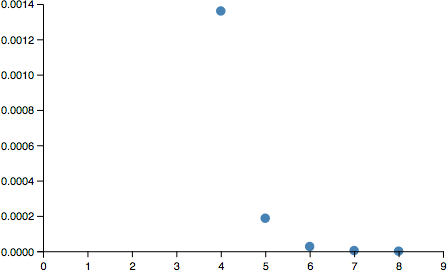
\includegraphics[scale=0.65]{improper-integrals-error.png}
\caption{Error for $n=4,5,6,7,8$.}
\end{figure}

We can see that our error decreases for larger values of $n$ and
approaches $0$ quickly. Even for $n=4$ it's accurate.
}
